\documentclass{beamer}
\usepackage{graphicx}
\usepackage{booktabs} % For better table rules
\usepackage{amsmath} % For math symbols
% Choose a theme
\usetheme{Madrid}


\title{Decoding Student Retention and Churn of Vodafone (Telecel) in KNUST}
\subtitle{A Survival Analysis Approach}
\author{Musah Faridu Oubda
	\\ Kassim Asana
	\\ Sarpong Linda
	\\ Torsi Edmond Collins
	\\ Asiamah Ezekiel}

\institute{Kwame Nkrumah University of Science and Technology}
\date{\today}

\begin{document}
	% Title page
	\begin{frame}
		\titlepage
	\end{frame}
	
	% Table of contents
	\begin{frame}{OUTLINE}
		\tableofcontents
	\end{frame}
	
	
	\section{Introduction}
	
	\begin{frame}
		\frametitle{BACKGROUND OF STUDY}
		\begin{itemize}
			
			
			\item 	The Ghanaian telecommunications industry, particularly Vodafone (now Telecel), faces significant challenges with customer churn. 
   \item Retaining customers is crucial for profitability, especially in a highly competitive market where acquiring new customers is more expensive than retaining existing ones.

			\item 	Telecel, which acquired Vodafone in early 2023, aims to enhance service offerings and improve customer retention. The study focuses on understanding and addressing student churn at KNUST using survival analysis methods to develop strategies for reducing churn and improving customer satisfaction.
			
		\end{itemize}
	\end{frame}
	
	\begin{frame}
		\frametitle{PROBLEM STATEMENT}
		\begin{itemize}
			\item This research aims to investigate the factors contributing to student churn develop a survival analysis model for detecting at-risk students and design specific strategies to improve retention rates. 

			\item It also seeks to enhance Telecel’s services, improve student experience, and foster long-term relationships between Vodafone (Telecel) and KNUST.
			
			
		\end{itemize}
	\end{frame}
	
	\begin{frame}
		\frametitle{RESEARCH OBJECTIVES}
		\begin{itemize}
			\item  To identify critical academic years when students are more likely to churn.

			\item To provide Telecel insights into students' churn patterns.
		\end{itemize}
    
    \end{frame}
	\section{Methodology}
	
	
	
	\begin{frame}
		\frametitle{METHODOLOGY}
		\begin{itemize}
			\item The data was collected via a survey, through Google Forms capturing specific aspects relevant to the study while ensuring confidentiality and ethical consideration
		
			\item Level 400 students in College of Science are the targeted audience. 
			\item The sample size was determined through simple random sampling targeting approximately 338 students from a population of about 2835.
   	\end{itemize}
    \end{frame}


	\begin{frame}
		\frametitle{METHODOLOGY}
\begin{figure}
    \centering
      \caption{Methodology}
    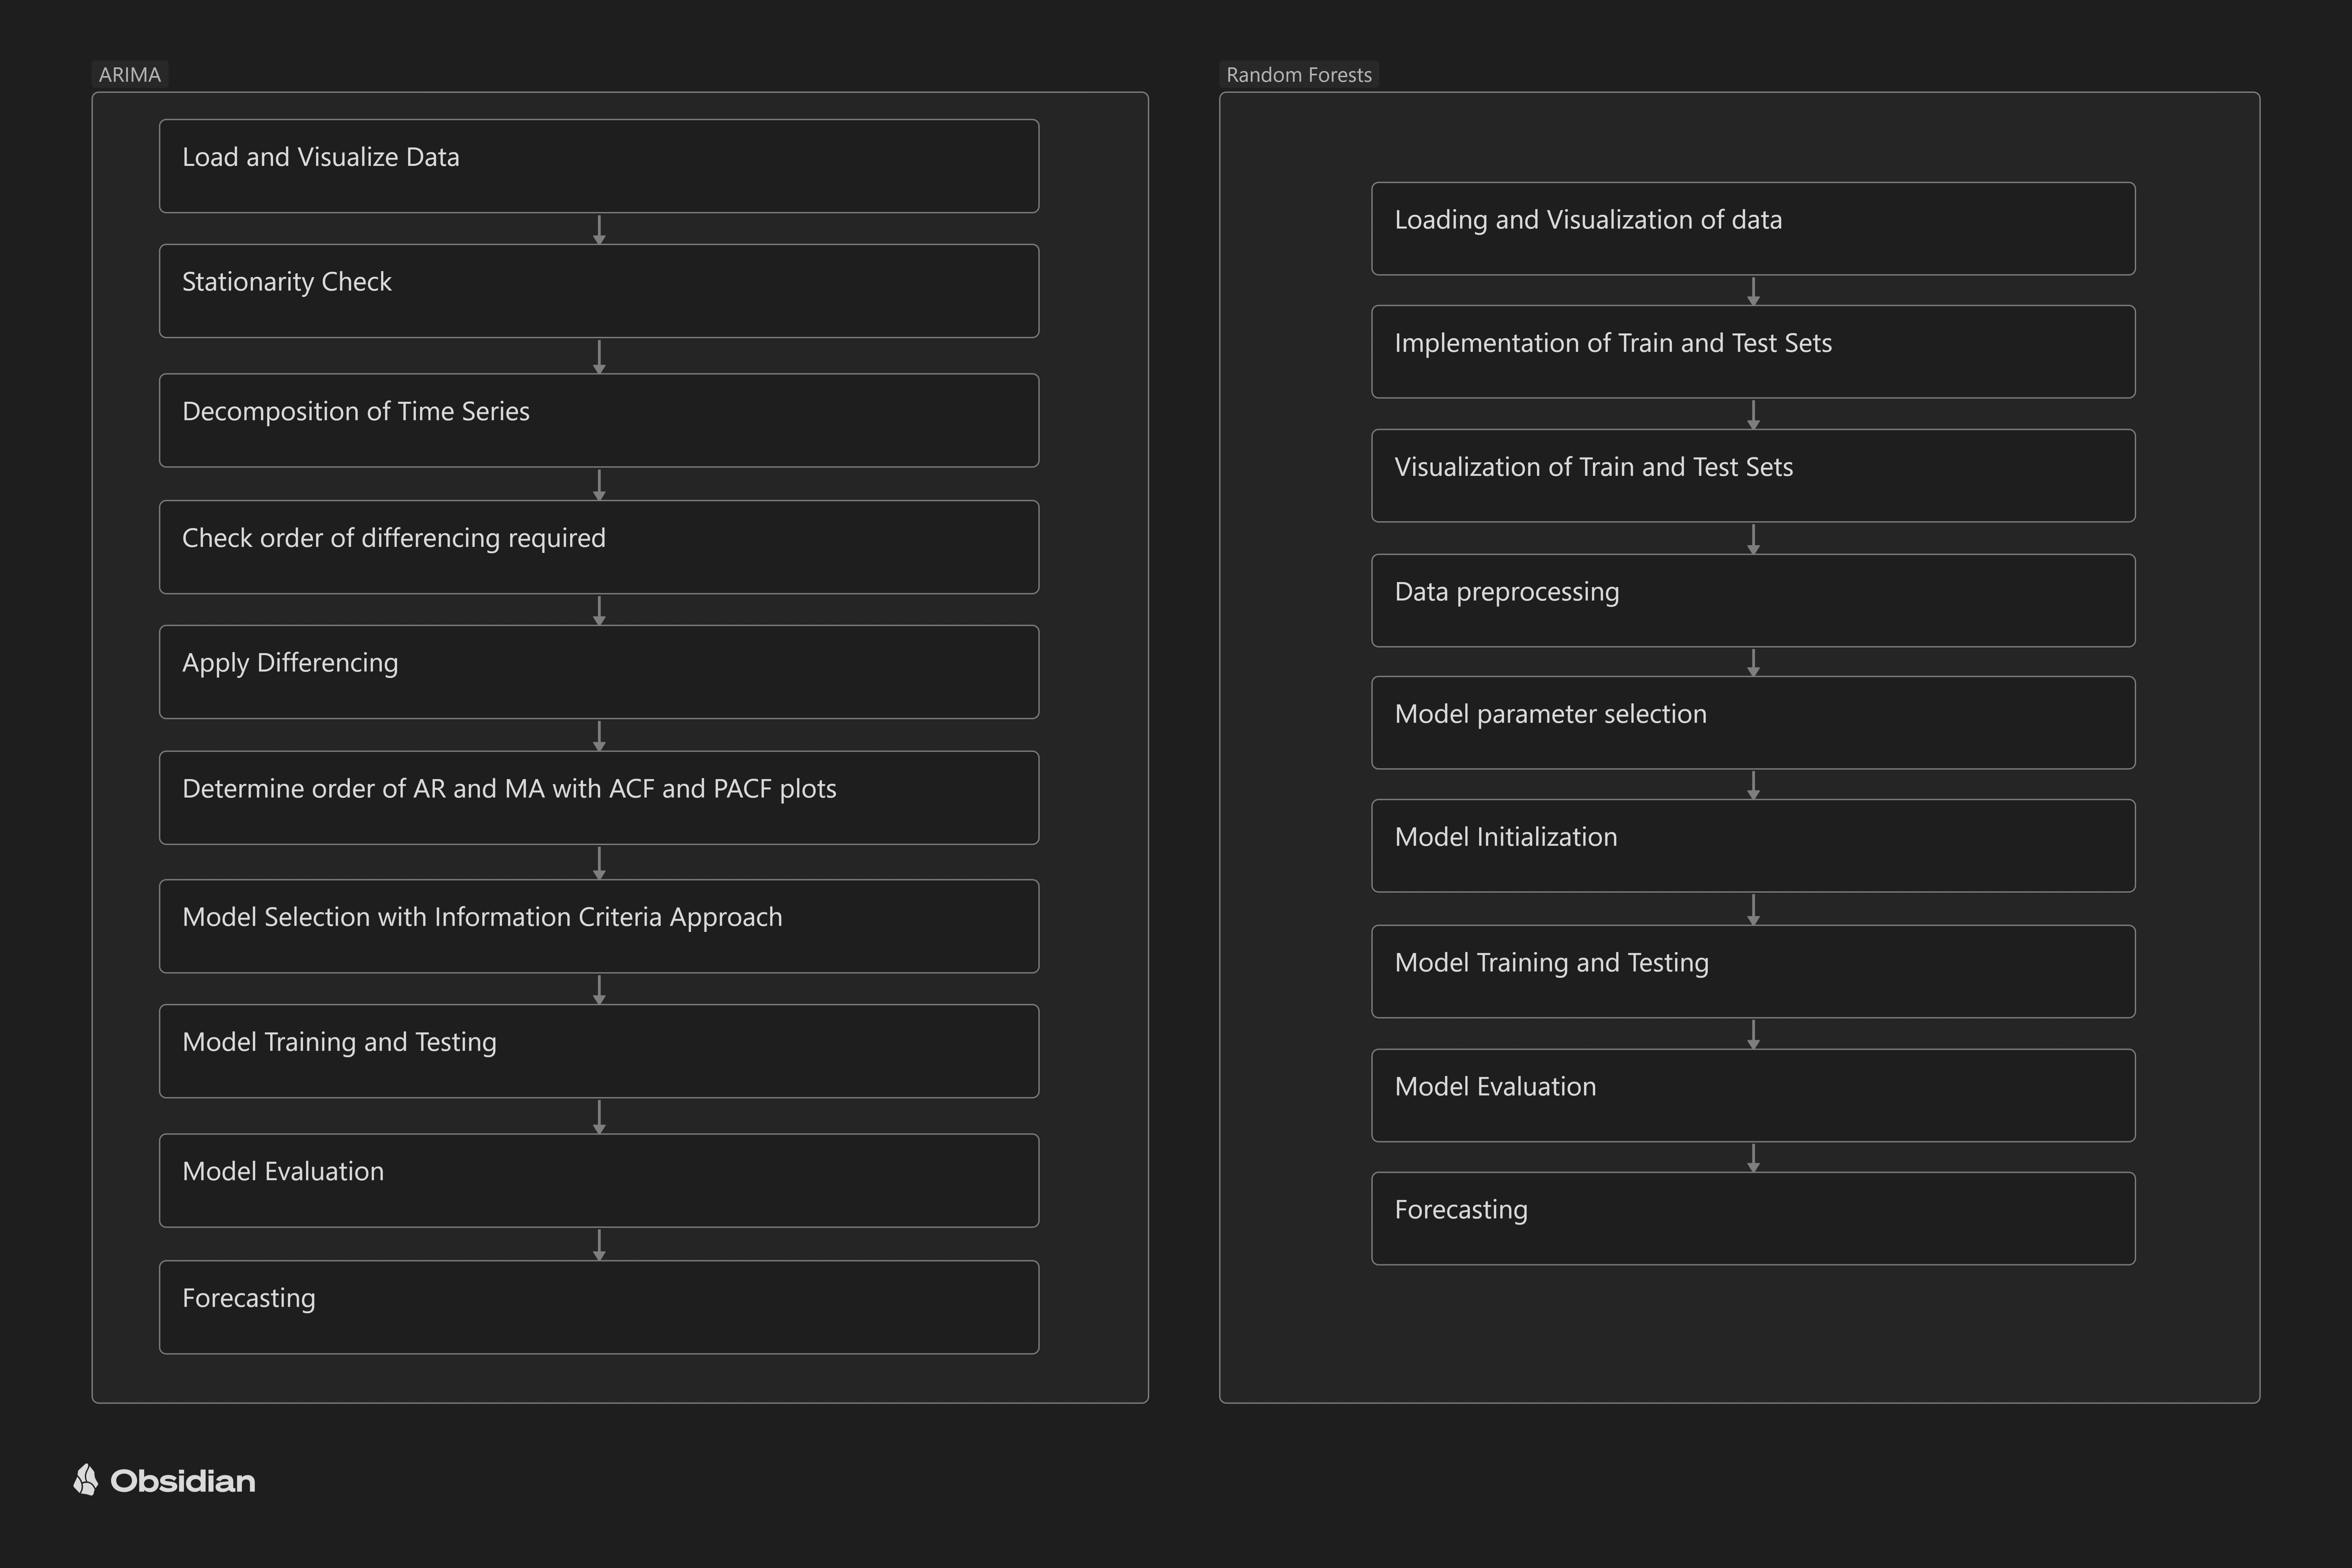
\includegraphics[width=0.65\linewidth]{Presentation/Methodology.png}
  
    \label{fig:enter-label}
\end{figure}

	\end{frame}
	
	\begin{frame}
    \frametitle{DATA DESCRIPTION}
  \begin{figure}
      \centering
      \includegraphics[width=0.75\linewidth]{Presentation/Description of Variables.png}
      \caption{Description of Variables}
      \label{fig:enter-label}
  \end{figure}
  
\end{frame}

 
	
	
	\section{Analysis and Findings}
	\begin{frame}
		\frametitle{KAPLAN  MEIER}
		\begin{figure}[H]
			\centering
			\includegraphics[width=0.47\textwidth]{Figure 4/4.1.png}
			\hfill
			\caption{KM Curve}
			\label{Table 1}
			\includegraphics[width=0.7\textwidth]{Presentation/ana.png}
			
			\caption{KM Analysis}
			\label{Figure 1}
		\end{figure}
	\end{frame}
	\begin{frame}
 		\frametitle{ACCELATED FAILURE RIME}
        
\begin{table}[H]
    \centering
    \begin{tabular}{lccc}
        \toprule
        Model & AIC & BIC & Hanna-Quinn \\
        \midrule
        WeibullAFTFitter & 182.568721 & 187.779061 & 32.486525 \\
        LogNormalAFTFitter & 175.138211 & 180.348551 & 32.486525 \\
        LogLogisticAFTFitter & 176.518119 & 181.728460 & 32.486525 \\
        \bottomrule
    \end{tabular}
    \caption{Model Comparison Metrics}
    \label{tab:model_comparison}
\end{table}

\noindent
\textbf{Results:} \\
The AFT model with the lowest AIC is: \textit{LogNormalAFTFitter} \\
The AFT model with the lowest BIC is: \textit{LogNormalAFTFitter} \\
The AFT model with the lowest Hanna-Quinn is: \textit{WeibullAFTFitter}

    \end{frame}
	
	\begin{frame}
		\frametitle{ANALYSIS AND FINDINGS}
		\begin{figure}
			\centering
			\includegraphics[width=0.75\linewidth]{Presentation/cox and weilbull.png}
			\caption{Cox and Lognormal Analysis}
			\label{Figure 2}
		\end{figure}
	\end{frame}
	
	
	\begin{frame}
		\frametitle{ANALYSIS AND FINDINGS CON'T}
		\begin{figure}[H]
			\centering
			\begin{minipage}{0.8\textwidth}
				\centering
				\includegraphics[width=\textwidth]{Figure 4/4.2.png}
				\caption{Cox Coefficients}
				\label{Figure 3}
			\end{minipage}\hfill
		
		\end{figure}
	\end{frame}
		\begin{frame}
		\frametitle{ANALYSIS AND FINDINGS CON'T}
		\begin{figure}[H]
			\centering
			\begin{minipage}{0.8\textwidth}
				\centering
				\includegraphics[width=\textwidth]{Figure 4/4.4.png}
				\caption{LogNormal Coefficients}
				\label{Figure 4}
				
			\end{minipage}
    
		\end{frame}
  

	\begin{frame}
		\frametitle{MODEL COMPARISON}
		%Table here
		\begin{table}[H]
			\centering
			\begin{tabular}{lcc}
				\toprule
				\textbf{Model} & \textbf{Concordance} & \textbf{AIC} \\
				\midrule
				LogNormal& 0.767& 169.052\\
				Cox PH & 0.74& 174.41\\
				\bottomrule
			\end{tabular}
			\caption{Model Concordance and AIC values}
			\label{Table 2}
			
		\end{table}
		
	\end{frame}
	
	\section{Conclusion}
	
	\begin{frame}
		\frametitle{CONCLUSION}
		\begin{itemize}
			\item The research shows that Lognormal AFT is the best model.
			\item Poor Network Quality is the covariate that tends to increase the rate at which students churn the most 
   \item  Residence increases the time to the event of churn happening the most.
   \item Data Exhaustion is the covariate that is most significant to the study.
			\item Students tend to churn at the end of their second year.
		\end{itemize}
	\end{frame}
 
	
	\begin{frame}
		\frametitle{RECOMMENDATIONS}
		\begin{itemize}
			\item Conduct regular surveys.
			\item Enhance the quality and reliability of network coverage across KNUST to reduce churn rates.
			\item Improve the responsiveness and quality of customer support to address student concerns more effectively.

			
		\end{itemize}
	\end{frame}
 
	
	\begin{frame}
		%\frametitle{}
		\centering{ THANK YOU}
		
		
		
	\end{frame}
	
\end{document}

